\documentclass{standalone}

\usepackage{standalone}
\standaloneconfig{mode=image|tex}

%\usepackage{geometry}
%\geometry{
%paperwidth=20cm,
%paperheight=20cm,
%margin=0.01cm
%}


% AMS Packages
\usepackage{amsmath}
\usepackage{amsthm}
\usepackage{amssymb}

\usepackage[utf8]{inputenc}
\usepackage{graphicx}
\usepackage{color}
\usepackage{multirow}
\usepackage{rotating}
\usepackage{bm}
\usepackage{xcolor}
\usepackage{tabu}
\usepackage[most]{tcolorbox}


%\usepackage[percent]{overpic}
\usepackage{tikz}
\usetikzlibrary{positioning,fit}
\usetikzlibrary{matrix}
\usetikzlibrary{calc}
\usepackage{ifthen}
\usepackage{pgf}
\usepackage{pgffor}
\usepgfmodule{shapes}
\usepgfmodule{plot}
\usetikzlibrary{decorations}
\usetikzlibrary{arrows}
\usetikzlibrary{snakes}
\usepackage{pgfplots}

\usepackage{array}
\newcolumntype{P}[1]{>{\centering\arraybackslash}p{#1}}
\newcolumntype{M}[1]{>{\centering\arraybackslash}m{#1}}

\usepackage[T1]{fontenc}
\usepackage{helvet}
\renewcommand{\familydefault}{\sfdefault}
\usepackage[helvet]{sfmath}
\everymath={\sf}


\newcommand{\eg}{\textit{e.g.,}\ }
\newcommand{\ie}{\textit{i.e.,}\ }
\newcommand{\cf}{\textit{cf.}\ }
\newcommand{\etal}{\textit{et al.}}


\setlength{\tabcolsep}{1pt}
\def\arraystretch{1.05}

\fboxsep=0mm % Padding thickness
\fboxrule=1pt % Border thickness

\newcommand{\converged}{\colorbox{white!30}{\textcolor{white}{\textbf{Converged}}}}
%\newcommand{\converged}{\colorbox{red!30}{\textbf{Converged}}}
%\newcommand{\converged}{\footnotesize\textbf{Convergence}}
%\newcommand{\convergedFstLine}{\textbf{Converged}}
\newcommand{\convergedFstLine}{\colorbox{white!30}{\textcolor{white}{\textbf{Converged}}}}
\newcommand{\convergedFstCol}{\textbf{Converged}}
\newcommand{\notconverged}{\colorbox{white!30}{\textcolor{white}{\textbf{Converged}}}}
\newcommand{\ignored}{Ignored}


\newcommand{\convergedBox}[1]{%
    \begin{tcolorbox}[colframe=black,colback=white,boxrule=1.3pt,arc=3pt,left=2pt,right=2pt,top=2pt,bottom=2pt,boxsep=0pt]
        #1
    \end{tcolorbox}
}


\newcommand{\notconvergedBox}[1]{%
    \begin{tcolorbox}[colframe=white,colback=white,boxrule=1.3pt,arc=3pt,left=2pt,right=2pt,top=2pt,bottom=2pt,boxsep=0pt]
        #1
    \end{tcolorbox}
}

\newcommand{\ignoredBox}[1]{%
    \begin{tcolorbox}[colframe=gray,colback=white,frame style={pattern=dot},boxrule=1.3pt,arc=3pt,left=2pt,right=2pt,top=2pt,bottom=2pt,boxsep=0pt]
        \begin{tikzpicture}[line width=0pt]
            \begin{scope}[blend group=multiply]
                \node[inner sep=0] (ignoredImg) at (0,0) {#1};
                %\fill[white!50!black] (0,0) ++(-.5,-.5) rectangle ++(1,1);
                \fill [draw=none, fill=black, fill opacity=0.3] (ignoredImg.north west) -- (ignoredImg.north east) -- (ignoredImg.south east) -- (ignoredImg.south west) -- (ignoredImg.north west) -- cycle;
            \end{scope}
        \end{tikzpicture}
    \end{tcolorbox}
}

\newcommand\includegraphicsie[2][width=\linewidth]{\IfFileExists{#2}{\includegraphics[#1]{#2}}{\includegraphics[draft,#1]{#2}}}


\begin{document}

\taburulecolor{white}
\setlength\arrayrulewidth{1.0pt}
%\begin{tabu}{@{} | M{2.0cm} M{2.0cm} M{2.0cm} M{2.0cm} M{2.0cm} M{2.0cm} M{2.0cm} M{2.0cm} M{2.0cm} |||| M{2.3cm}|| M{2.3cm}| @{}}
\begin{tabu}{@{} | M{2.0cm} M{2.0cm} M{2.0cm} M{2.0cm} M{2.0cm} M{2.0cm} |||| M{2.3cm} M{0.1cm} | @{}}
\hline


\multicolumn{7}{|c|}{
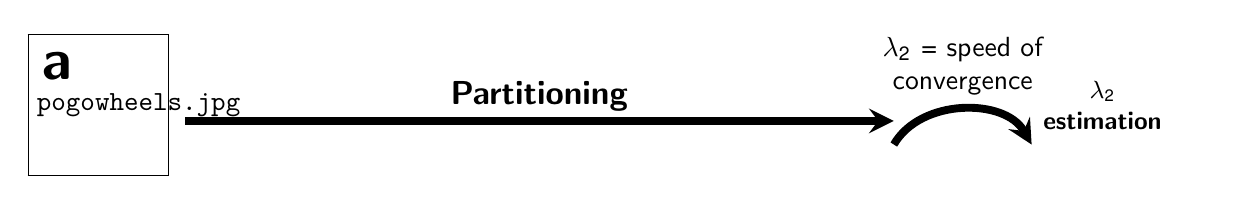
\begin{tikzpicture}
    \node[inner sep=0pt] (kilo) at (0.0,0.5) {\includegraphicsie[trim={0cm 0cm 0cm 0cm},clip,height=1.8cm]{pogowheels.jpg}};
    \node [above left=-0.70cm and -0.70cm of kilo] (a) {\huge \textbf{a}};
    
    \draw [-stealth, line width=0.10cm] (1.1,0.3) -- (10.1,0.3)  node [inner sep=2pt,pos=0.5,above,font=\large]{\textbf{Partitioning}};
    %\draw [-stealth, line width=0.10cm] (11.15,0.3) -- (12.00,0.3) node [inner sep=2pt,pos=0.5,above,font=\large,align=center,text width=2.5cm]{\textbf{$\lambda_2$ estimation}};
    \node [inner sep=2pt,font=\small,align=center,text width=2.5cm] at (12.75, 0.5) {\textbf{$\lambda_2$\\estimation}};

    %\draw [-stealth, line width=0.10cm] (19,0) to [bend left=45] (21,0) node [inner sep=1pt,pos=0.5,above,font=\small]{TODO};
    \draw [-stealth, line width=0.10cm] (10.1,0) to [bend left=60] (11.85,0);
    \node [font=\normalsize,align=center,text width=2.5cm] (transition) at (10.975,1) {$\lambda_2 = $ speed of convergence};
\end{tikzpicture}
}


\\[0.0cm]


%\large Initial state
\multirow{2}{*}{\shortstack[|c]{\large Initial\\\large state}}
&
\multicolumn{5}{|c|}{\Large Time-lapse of $\texttt{sign}(s_i^{n})$ during one iteration} &
%\multirow{2}{*}{\shortstack[c]{\large Indiv. $\lambda_2$\\\large from one it.}} &
\multirow{2}{*}{\shortstack[|c]{\large Final $\lambda_2$\\\large after 1 it.}} \\

&
\normalsize $n=0$ & \normalsize $n=60$ & \normalsize $n=110$ & \normalsize $n=180$ & \normalsize $n=210$ & \\

\hline

    \raisebox{-0.5cm}{\notconvergedBox{ \includegraphicsie[trim={0cm 0cm 0cm 0cm},clip,width=1.8cm]{disk/2022-07-22_10-18-21/start.png}} } &
    \raisebox{-0.5cm}{\notconvergedBox{ \includegraphicsie[trim={0cm 0cm 0cm 0cm},clip,width=1.8cm]{disk/2022-07-22_10-18-21/n0.pdf}} } &
    \raisebox{-0.5cm}{\notconvergedBox{ \includegraphicsie[trim={0cm 0cm 0cm 0cm},clip,width=1.8cm]{disk/2022-07-22_10-18-21/n60.pdf}} } &
    \raisebox{-0.5cm}{\convergedBox{    \includegraphicsie[trim={0cm 0cm 0cm 0cm},clip,width=1.8cm]{disk/2022-07-22_10-18-21/n110.pdf}} } &
    \raisebox{-0.5cm}{\convergedBox{    \includegraphicsie[trim={0cm 0cm 0cm 0cm},clip,width=1.8cm]{disk/2022-07-22_10-18-21/n180.pdf}} } &
    \raisebox{-0.5cm}{\convergedBox{    \includegraphicsie[trim={0cm 0cm 0cm 0cm},clip,width=1.8cm]{disk/2022-07-22_10-18-21/n210.pdf}} } &
    \raisebox{-0.5cm}{\notconvergedBox{ \includegraphicsie[trim={0cm 0cm 0cm 0cm},clip,width=1.8cm]{disk/2022-07-22_10-18-21/lambda.pdf}} } &
    \hspace*{-0.5cm}\rotatebox{90}{\centering \large \textbf{Correct}}
    \\[0.0cm]
    &
    \notconverged &
    \notconverged &
    \convergedFstCol &
    \converged &
    \converged &
    \\[0.3cm]
    \hline


    \raisebox{-0.5cm}{\notconvergedBox{ \includegraphicsie[trim={0cm 0cm 0cm 0cm},clip,width=1.8cm]{disk/2022-07-21_14-16-04/start.png}} } &
    \raisebox{-0.5cm}{\notconvergedBox{ \includegraphicsie[trim={0cm 0cm 0cm 0cm},clip,width=1.8cm]{disk/2022-07-21_14-16-04/n0.pdf}} } &
    \raisebox{-0.5cm}{\notconvergedBox{ \includegraphicsie[trim={0cm 0cm 0cm 0cm},clip,width=1.8cm]{disk/2022-07-21_14-16-04/n60.pdf}} } &
    \raisebox{-0.5cm}{\convergedBox{    \includegraphicsie[trim={0cm 0cm 0cm 0cm},clip,width=1.8cm]{disk/2022-07-21_14-16-04/n110.pdf}} } &
    \raisebox{-0.5cm}{\convergedBox{    \includegraphicsie[trim={0cm 0cm 0cm 0cm},clip,width=1.8cm]{disk/2022-07-21_14-16-04/n180.pdf}} } &
    \raisebox{-0.5cm}{\convergedBox{    \includegraphicsie[trim={0cm 0cm 0cm 0cm},clip,width=1.8cm]{disk/2022-07-21_14-16-04/n210.pdf}} } &
    \raisebox{-0.5cm}{\notconvergedBox{ \includegraphicsie[trim={0cm 0cm 0cm 0cm},clip,width=1.8cm]{disk/2022-07-21_14-16-04/lambda.pdf}} } &
    \hspace*{-0.5cm}\rotatebox{90}{\centering \large \textbf{Correct}}
    \\[0.0cm]
    &
    \notconverged &
    \notconverged &
    \convergedFstCol &
    \converged &
    \converged &
    \\[0.3cm]
    \hline

    \raisebox{-0.5cm}{\notconvergedBox{ \includegraphicsie[trim={0cm 0cm 0cm 0cm},clip,width=1.8cm]{disk/2022-09-15_15-45-26/start.png}} } &
    \raisebox{-0.5cm}{\notconvergedBox{ \includegraphicsie[trim={0cm 0cm 0cm 0cm},clip,width=1.8cm]{disk/2022-09-15_15-45-26/n0.pdf}} } &
    \raisebox{-0.5cm}{\convergedBox{    \includegraphicsie[trim={0cm 0cm 0cm 0cm},clip,width=1.8cm]{disk/2022-09-15_15-45-26/n60.pdf}} } &
    \raisebox{-0.5cm}{\convergedBox{    \includegraphicsie[trim={0cm 0cm 0cm 0cm},clip,width=1.8cm]{disk/2022-09-15_15-45-26/n110.pdf}} } &
    \raisebox{-0.5cm}{\convergedBox{    \includegraphicsie[trim={0cm 0cm 0cm 0cm},clip,width=1.8cm]{disk/2022-09-15_15-45-26/n180.pdf}} } &
    \raisebox{-0.5cm}{\convergedBox{    \includegraphicsie[trim={0cm 0cm 0cm 0cm},clip,width=1.8cm]{disk/2022-09-15_15-45-26/n210.pdf}} } &
    \raisebox{-0.5cm}{\notconvergedBox{ \includegraphicsie[trim={0cm 0cm 0cm 0cm},clip,width=1.8cm]{disk/2022-09-15_15-45-26/lambda.pdf}} } &
    \hspace*{-0.5cm}\rotatebox{90}{\centering \large \textbf{Correct}}
    \\[0.0cm]
    &
    \notconverged &
    \convergedFstCol &
    \converged &
    \converged &
    \converged &
    \\[0.3cm]
    \hline



    \raisebox{-0.5cm}{\notconvergedBox{ \includegraphicsie[trim={0cm 0cm 0cm 0cm},clip,width=1.8cm]{disk/2022-07-21_15-47-12/start.png}} } &
    \raisebox{-0.5cm}{\notconvergedBox{ \includegraphicsie[trim={0cm 0cm 0cm 0cm},clip,width=1.8cm]{disk/2022-07-21_15-47-12/n0.pdf}} } &
    \raisebox{-0.5cm}{\notconvergedBox{ \includegraphicsie[trim={0cm 0cm 0cm 0cm},clip,width=1.8cm]{disk/2022-07-21_15-47-12/n60.pdf}} } &
    \raisebox{-0.5cm}{\convergedBox{    \includegraphicsie[trim={0cm 0cm 0cm 0cm},clip,width=1.8cm]{disk/2022-07-21_15-47-12/n110.pdf}} } &
    \raisebox{-0.5cm}{\convergedBox{    \includegraphicsie[trim={0cm 0cm 0cm 0cm},clip,width=1.8cm]{disk/2022-07-21_15-47-12/n180.pdf}} } &
    \raisebox{-0.5cm}{\convergedBox{    \includegraphicsie[trim={0cm 0cm 0cm 0cm},clip,width=1.8cm]{disk/2022-07-21_15-47-12/n210.pdf}} } &
    \raisebox{-0.5cm}{\notconvergedBox{ \includegraphicsie[trim={0cm 0cm 0cm 0cm},clip,width=1.8cm]{disk/2022-07-21_15-47-12/lambda.pdf}} } &
    \hspace*{-0.5cm}\rotatebox{90}{\centering \large \textbf{Correct}}
    \\[0.0cm]
    &
    \notconverged &
    \notconverged &
    \convergedFstCol &
    \converged &
    \converged &
    \\[0.3cm]
    \hline


%    \raisebox{-0.5cm}{\notconvergedBox{ \includegraphicsie[trim={0cm 0cm 0cm 0cm},clip,width=1.8cm]{disk/2022-09-16_10-38-16/start.png}} } &
%    \raisebox{-0.5cm}{\notconvergedBox{ \includegraphicsie[trim={0cm 0cm 0cm 0cm},clip,width=1.8cm]{disk/2022-09-16_10-38-16/n0.pdf}} } &
%    \raisebox{-0.5cm}{\convergedBox{    \includegraphicsie[trim={0cm 0cm 0cm 0cm},clip,width=1.8cm]{disk/2022-09-16_10-38-16/n60.pdf}} } &
%    \raisebox{-0.5cm}{\convergedBox{    \includegraphicsie[trim={0cm 0cm 0cm 0cm},clip,width=1.8cm]{disk/2022-09-16_10-38-16/n110.pdf}} } &
%    \raisebox{-0.5cm}{\ignoredBox{      \includegraphicsie[trim={0cm 0cm 0cm 0cm},clip,width=1.8cm]{disk/2022-09-16_10-38-16/n180.pdf}} } &
%    \raisebox{-0.5cm}{\ignoredBox{      \includegraphicsie[trim={0cm 0cm 0cm 0cm},clip,width=1.8cm]{disk/2022-09-16_10-38-16/n210.pdf}} } &
%    \raisebox{-0.5cm}{\notconvergedBox{ \includegraphicsie[trim={0cm 0cm 0cm 0cm},clip,width=1.8cm]{disk/2022-09-16_10-38-16/lambda.pdf}} } &
%    \hspace*{-0.5cm}\rotatebox{90}{\centering \large \textbf{Correct}}
%    \\[0.0cm]
%    &
%    \notconverged &
%    \convergedFstCol &
%    \converged &
%    \ignored &
%    \ignored &
%    \\[0.3cm]
%    \hline


    \raisebox{-0.5cm}{\notconvergedBox{ \includegraphicsie[trim={0cm 0cm 0cm 0cm},clip,width=1.8cm]{disk/2022-07-22_13-33-07/start.png}} } &
    \raisebox{-0.5cm}{\notconvergedBox{ \includegraphicsie[trim={0cm 0cm 0cm 0cm},clip,width=1.8cm]{disk/2022-07-22_13-33-07/n0.pdf}} } &
    \raisebox{-0.5cm}{\convergedBox{    \includegraphicsie[trim={0cm 0cm 0cm 0cm},clip,width=1.8cm]{disk/2022-07-22_13-33-07/n60.pdf}} } &
    \raisebox{-0.5cm}{\convergedBox{    \includegraphicsie[trim={0cm 0cm 0cm 0cm},clip,width=1.8cm]{disk/2022-07-22_13-33-07/n110.pdf}} } &
    \raisebox{-0.5cm}{\convergedBox{    \includegraphicsie[trim={0cm 0cm 0cm 0cm},clip,width=1.8cm]{disk/2022-07-22_13-33-07/n180.pdf}} } &
    \raisebox{-0.5cm}{\convergedBox{    \includegraphicsie[trim={0cm 0cm 0cm 0cm},clip,width=1.8cm]{disk/2022-07-22_13-33-07/n210.pdf}} } &
    \raisebox{-0.5cm}{\notconvergedBox{ \includegraphicsie[trim={0cm 0cm 0cm 0cm},clip,width=1.8cm]{disk/2022-07-22_13-33-07/lambda.pdf}} } &
    \hspace*{-0.5cm}\rotatebox{90}{\centering \large \textbf{Correct}}
    \\[0.0cm]
    &
    \notconverged &
    \convergedFstCol &
    \converged &
    \converged &
    \converged &
    \\[0.3cm]
    \hline


    \raisebox{-0.5cm}{\notconvergedBox{ \includegraphicsie[trim={0cm 0cm 0cm 0cm},clip,width=1.8cm]{disk/2022-07-22_17-06-29/start.png}} } &
    \raisebox{-0.5cm}{\notconvergedBox{ \includegraphicsie[trim={0cm 0cm 0cm 0cm},clip,width=1.8cm]{disk/2022-07-22_17-06-29/n0.pdf}} } &
    \raisebox{-0.5cm}{\notconvergedBox{ \includegraphicsie[trim={0cm 0cm 0cm 0cm},clip,width=1.8cm]{disk/2022-07-22_17-06-29/n60.pdf}} } &
    \raisebox{-0.5cm}{\convergedBox{    \includegraphicsie[trim={0cm 0cm 0cm 0cm},clip,width=1.8cm]{disk/2022-07-22_17-06-29/n110.pdf}} } &
    \raisebox{-0.5cm}{\convergedBox{    \includegraphicsie[trim={0cm 0cm 0cm 0cm},clip,width=1.8cm]{disk/2022-07-22_17-06-29/n180.pdf}} } &
    \raisebox{-0.5cm}{\convergedBox{    \includegraphicsie[trim={0cm 0cm 0cm 0cm},clip,width=1.8cm]{disk/2022-07-22_17-06-29/n210.pdf}} } &
    \raisebox{-0.5cm}{\notconvergedBox{ \includegraphicsie[trim={0cm 0cm 0cm 0cm},clip,width=1.8cm]{disk/2022-07-22_17-06-29/lambda.pdf}} } &
    \hspace*{-0.5cm}\rotatebox{90}{\centering \large \textbf{Correct}}
    \\[0.0cm]
    &
    \notconverged &
    \notconverged &
    \convergedFstCol &
    \converged &
    \converged &
    \\[0.3cm]
    \hline




%    \raisebox{-0.5cm}{\notconvergedBox{ \includegraphicsie[trim={0cm 0cm 0cm 0cm},clip,width=1.8cm]{disk/2022-07-22_11-50-10/start.png}} } &
%    \raisebox{-0.5cm}{\notconvergedBox{ \includegraphicsie[trim={0cm 0cm 0cm 0cm},clip,width=1.8cm]{disk/2022-07-22_11-50-10/n0.pdf}} } &
%    \raisebox{-0.5cm}{\convergedBox{    \includegraphicsie[trim={0cm 0cm 0cm 0cm},clip,width=1.8cm]{disk/2022-07-22_11-50-10/n60.pdf}} } &
%    \raisebox{-0.5cm}{\convergedBox{    \includegraphicsie[trim={0cm 0cm 0cm 0cm},clip,width=1.8cm]{disk/2022-07-22_11-50-10/n110.pdf}} } &
%    \raisebox{-0.5cm}{\ignoredBox{      \includegraphicsie[trim={0cm 0cm 0cm 0cm},clip,width=1.8cm]{disk/2022-07-22_11-50-10/n180.pdf}} } &
%    \raisebox{-0.5cm}{\ignoredBox{      \includegraphicsie[trim={0cm 0cm 0cm 0cm},clip,width=1.8cm]{disk/2022-07-22_11-50-10/n210.pdf}} } &
%    \raisebox{-0.5cm}{\notconvergedBox{ \includegraphicsie[trim={0cm 0cm 0cm 0cm},clip,width=1.8cm]{disk/2022-07-22_11-50-10/lambda.pdf}} } &
%    \hspace*{-0.5cm}\rotatebox{90}{\centering \large Incorrect}
%    \\[0.0cm]
%    &
%    \notconverged &
%    \convergedFstCol &
%    \converged &
%    \ignored &
%    \ignored &
%    \\[0.3cm]
%    \hline


    \raisebox{-0.5cm}{\notconvergedBox{ \includegraphicsie[trim={0cm 0cm 0cm 0cm},clip,width=1.8cm]{disk/2022-09-19_16-58-24/start.png}} } &
    \raisebox{-0.5cm}{\notconvergedBox{ \includegraphicsie[trim={0cm 0cm 0cm 0cm},clip,width=1.8cm]{disk/2022-09-19_16-58-24/n0.pdf}} } &
    \raisebox{-0.5cm}{\notconvergedBox{ \includegraphicsie[trim={0cm 0cm 0cm 0cm},clip,width=1.8cm]{disk/2022-09-19_16-58-24/n60.pdf}} } &
    \raisebox{-0.5cm}{\convergedBox{    \includegraphicsie[trim={0cm 0cm 0cm 0cm},clip,width=1.8cm]{disk/2022-09-19_16-58-24/n110.pdf}} } &
    \raisebox{-0.5cm}{\convergedBox{    \includegraphicsie[trim={0cm 0cm 0cm 0cm},clip,width=1.8cm]{disk/2022-09-19_16-58-24/n180.pdf}} } &
    \raisebox{-0.5cm}{\convergedBox{    \includegraphicsie[trim={0cm 0cm 0cm 0cm},clip,width=1.8cm]{disk/2022-09-19_16-58-24/n210.pdf}} } &
    \raisebox{-0.5cm}{\notconvergedBox{ \includegraphicsie[trim={0cm 0cm 0cm 0cm},clip,width=1.8cm]{disk/2022-09-19_16-58-24/lambda.pdf}} } &
    \hspace*{-0.5cm}\rotatebox{90}{\centering \large Incorrect}
    \\[0.0cm]
    &
    \notconverged &
    \notconverged &
    \convergedFstCol &
    \converged &
    \converged &
    \\[0.3cm]
    \hline


    \raisebox{-0.5cm}{\notconvergedBox{ \includegraphicsie[trim={0cm 0cm 0cm 0cm},clip,width=1.8cm]{disk/2022-09-19_10-41-44/start.png}} } &
    \raisebox{-0.5cm}{\notconvergedBox{ \includegraphicsie[trim={0cm 0cm 0cm 0cm},clip,width=1.8cm]{disk/2022-09-19_10-41-44/n0.pdf}} } &
    \raisebox{-0.5cm}{\notconvergedBox{ \includegraphicsie[trim={0cm 0cm 0cm 0cm},clip,width=1.8cm]{disk/2022-09-19_10-41-44/n60.pdf}} } &
    \raisebox{-0.5cm}{\convergedBox{    \includegraphicsie[trim={0cm 0cm 0cm 0cm},clip,width=1.8cm]{disk/2022-09-19_10-41-44/n110.pdf}} } &
    \raisebox{-0.5cm}{\convergedBox{    \includegraphicsie[trim={0cm 0cm 0cm 0cm},clip,width=1.8cm]{disk/2022-09-19_10-41-44/n180.pdf}} } &
    \raisebox{-0.5cm}{\convergedBox{    \includegraphicsie[trim={0cm 0cm 0cm 0cm},clip,width=1.8cm]{disk/2022-09-19_10-41-44/n210.pdf}} } &
    \raisebox{-0.5cm}{\notconvergedBox{ \includegraphicsie[trim={0cm 0cm 0cm 0cm},clip,width=1.8cm]{disk/2022-09-19_10-41-44/lambda.pdf}} } &
    \hspace*{-0.5cm}\rotatebox{90}{\centering \large Incorrect}
    \\[0.0cm]
    &
    \notconverged &
    \notconverged &
    \convergedFstCol &
    \converged &
    \converged &
    \\[0.3cm]
    \hline



\multicolumn{2}{|c|}{
\raisebox{0.1\height}{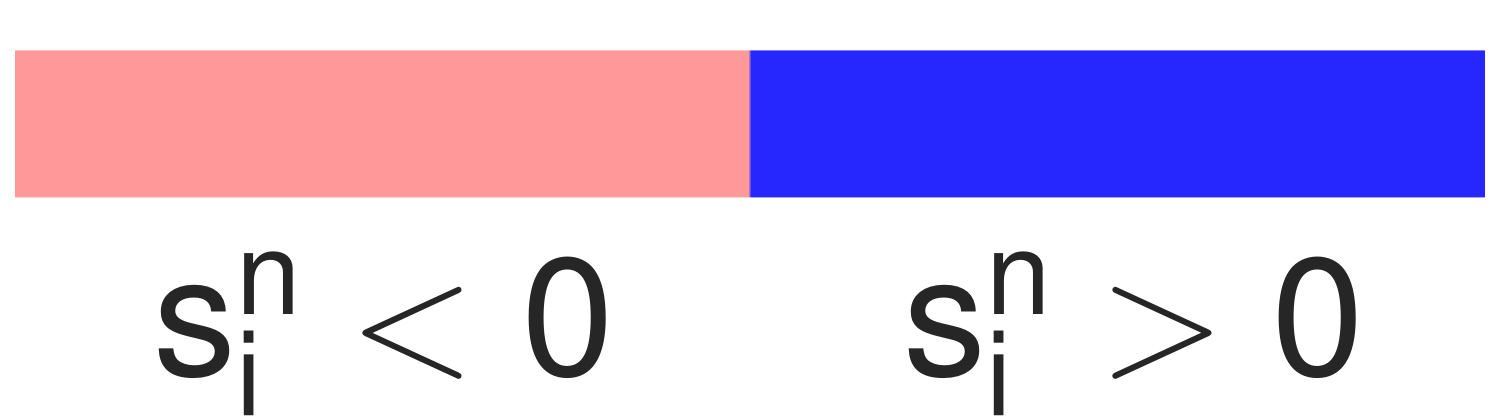
\includegraphics[trim=0 0 0 -2,width=4.0cm]{small_sign_s_cbar.png}}
}&
\multicolumn{2}{|c|}{
\raisebox{0.00\height}{
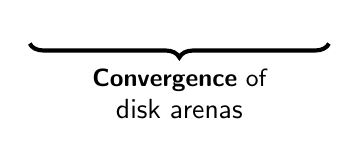
\begin{tikzpicture}[ultra thick]
\draw [decorate, decoration = {brace,raise=5pt,amplitude=5pt},line width=1.50pt]  (4.0,1.0) -- (0.2,1.0) node[pos=0.50,below=10pt,black]{\shortstack[c]{\small \textbf{Convergence} of\\disk arenas}};
\end{tikzpicture}}
}
& \multicolumn{2}{|c|}{
%\raisebox{0.1\height}{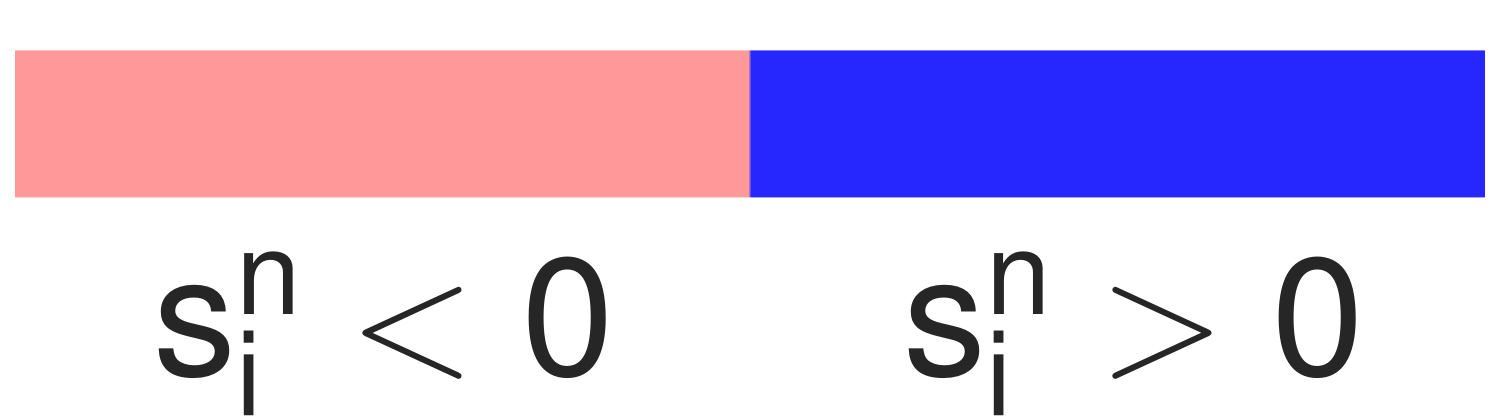
\includegraphics[trim=0 0 0 -2,width=4.0cm]{small_sign_s_cbar.png}}
%\hspace{-0.50cm}
\raisebox{-0.1\height}{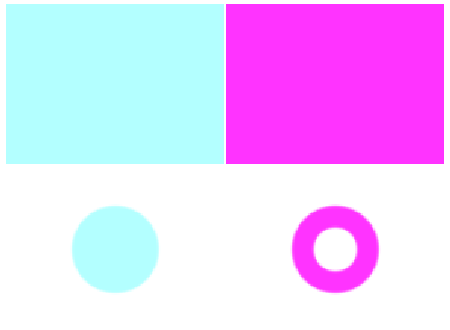
\includegraphics[trim=0 0 0 -2,width=2.0cm]{lambda_cbar.pdf}}
}
& \multicolumn{1}{|c|}{
\hspace{-0.50cm}
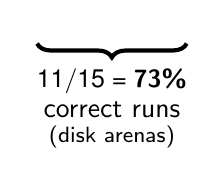
\begin{tikzpicture}[ultra thick]
%\draw [decorate, decoration = {brace,raise=5pt,amplitude=5pt},line width=1.50pt]  (2.2,1) -- (0.3,1) node[pos=0.50,below=10pt,black]{\shortstack[c]{\small Accuracy =\\\textbf{73\%} (30 runs)}};
\draw [decorate, decoration = {brace,raise=5pt,amplitude=5pt},line width=1.50pt]  (2.2,1) -- (0.3,1) node[pos=0.50,below=10pt,black]{\shortstack[c]{\small $11/15 = \textbf{73\%}$\\correct runs\\\footnotesize(disk arenas)}};
\end{tikzpicture}
}
\\[0cm]



\hline
\end{tabu}


\hspace{0.50cm}

\taburulecolor{white}
\setlength\arrayrulewidth{1.0pt}
%\begin{tabu}{@{} | M{2.0cm} M{2.0cm} M{2.0cm} M{2.0cm} M{2.0cm} M{2.0cm} M{2.0cm} M{2.0cm} M{2.0cm} |||| M{2.3cm}|| M{2.3cm}| @{}}
\begin{tabu}{@{} | M{2.0cm} M{2.0cm} M{2.0cm} M{2.0cm} M{2.0cm} M{2.0cm} |||| M{2.3cm} M{0.1cm} | @{}}
\hline


\multicolumn{7}{|c|}{
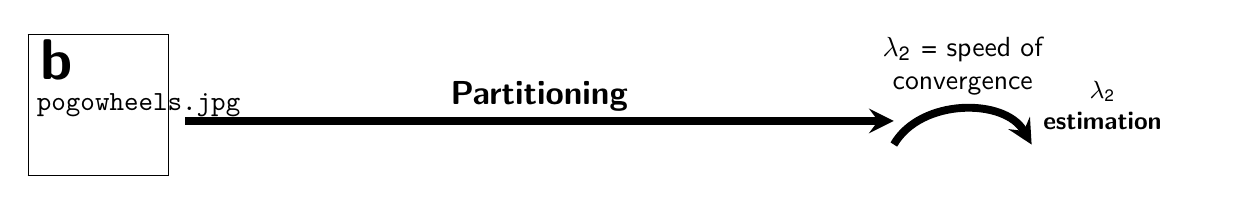
\begin{tikzpicture}
    \node[inner sep=0pt] (kilo) at (0.0,0.5) {\includegraphicsie[trim={0cm 0cm 0cm 0cm},clip,height=1.8cm]{pogowheels.jpg}};
    \node [above left=-0.70cm and -0.70cm of kilo] (b) {\huge \textbf{b}};
    
    \draw [-stealth, line width=0.10cm] (1.1,0.3) -- (10.1,0.3)  node [inner sep=2pt,pos=0.5,above,font=\large]{\textbf{Partitioning}};
    %\draw [-stealth, line width=0.10cm] (11.15,0.3) -- (12.00,0.3) node [inner sep=2pt,pos=0.5,above,font=\large,align=center,text width=2.5cm]{\textbf{$\lambda_2$ estimation}};
    \node [inner sep=2pt,font=\small,align=center,text width=2.5cm] at (12.75, 0.5) {\textbf{$\lambda_2$\\estimation}};

    %\draw [-stealth, line width=0.10cm] (19,0) to [bend left=45] (21,0) node [inner sep=1pt,pos=0.5,above,font=\small]{TODO};
    \draw [-stealth, line width=0.10cm] (10.1,0) to [bend left=60] (11.85,0);
    \node [font=\normalsize,align=center,text width=2.5cm] (transition) at (10.975,1) {$\lambda_2 = $ speed of convergence};
\end{tikzpicture}
}


\\[0.0cm]


\multirow{2}{*}{\shortstack[|c]{\large Initial\\\large state}}
&
\multicolumn{5}{|c|}{\Large Time-lapse of $\texttt{sign}(s_i^{n})$ during one iteration} &
\multirow{2}{*}{\shortstack[|c]{\large Final $\lambda_2$\\\large after 1 it.}} \\

&
\normalsize $n=0$ & \normalsize $n=60$ & \normalsize $n=110$ & \normalsize $n=180$ & \normalsize $n=210$ & \\

\hline

    \raisebox{-0.5cm}{\notconvergedBox{ \includegraphicsie[trim={0cm 0cm 0cm 0cm},clip,width=1.8cm]{annulus/2022-07-21_14-16-04/start.png}} } &
    \raisebox{-0.5cm}{\notconvergedBox{ \includegraphicsie[trim={0cm 0cm 0cm 0cm},clip,width=1.8cm]{annulus/2022-07-21_14-16-04/n0.pdf}} } &
    \raisebox{-0.5cm}{\notconvergedBox{ \includegraphicsie[trim={0cm 0cm 0cm 0cm},clip,width=1.8cm]{annulus/2022-07-21_14-16-04/n60.pdf}} } &
    \raisebox{-0.5cm}{\notconvergedBox{ \includegraphicsie[trim={0cm 0cm 0cm 0cm},clip,width=1.8cm]{annulus/2022-07-21_14-16-04/n110.pdf}} } &
    \raisebox{-0.5cm}{\convergedBox{    \includegraphicsie[trim={0cm 0cm 0cm 0cm},clip,width=1.8cm]{annulus/2022-07-21_14-16-04/n180.pdf}} } &
    \raisebox{-0.5cm}{\convergedBox{    \includegraphicsie[trim={0cm 0cm 0cm 0cm},clip,width=1.8cm]{annulus/2022-07-21_14-16-04/n210.pdf}} } &
    \raisebox{-0.5cm}{\notconvergedBox{ \includegraphicsie[trim={0cm 0cm 0cm 0cm},clip,width=1.8cm]{annulus/2022-07-21_14-16-04/lambda.pdf}} } &
    \hspace*{-0.5cm}\rotatebox{90}{\centering \large \textbf{Correct}}
    \\[0.0cm]
    &
    \notconverged &
    \notconverged &
    \notconverged &
    \convergedFstCol &
    \converged &
    \\[0.3cm]
    \hline


    \raisebox{-0.5cm}{\notconvergedBox{ \includegraphicsie[trim={0cm 0cm 0cm 0cm},clip,width=1.8cm]{annulus/2022-09-16_10-38-16/start.png}} } &
    \raisebox{-0.5cm}{\notconvergedBox{ \includegraphicsie[trim={0cm 0cm 0cm 0cm},clip,width=1.8cm]{annulus/2022-09-16_10-38-16/n0.pdf}} } &
    \raisebox{-0.5cm}{\notconvergedBox{ \includegraphicsie[trim={0cm 0cm 0cm 0cm},clip,width=1.8cm]{annulus/2022-09-16_10-38-16/n60.pdf}} } &
    \raisebox{-0.5cm}{\notconvergedBox{ \includegraphicsie[trim={0cm 0cm 0cm 0cm},clip,width=1.8cm]{annulus/2022-09-16_10-38-16/n110.pdf}} } &
    \raisebox{-0.5cm}{\convergedBox{    \includegraphicsie[trim={0cm 0cm 0cm 0cm},clip,width=1.8cm]{annulus/2022-09-16_10-38-16/n180.pdf}} } &
    \raisebox{-0.5cm}{\convergedBox{    \includegraphicsie[trim={0cm 0cm 0cm 0cm},clip,width=1.8cm]{annulus/2022-09-16_10-38-16/n210.pdf}} } &
    \raisebox{-0.5cm}{\notconvergedBox{ \includegraphicsie[trim={0cm 0cm 0cm 0cm},clip,width=1.8cm]{annulus/2022-09-16_10-38-16/lambda.pdf}} } &
    \hspace*{-0.5cm}\rotatebox{90}{\centering \large \textbf{Correct}}
    \\[0.0cm]
    &
    \notconverged &
    \notconverged &
    \notconverged &
    \convergedFstCol &
    \converged &
    \\[0.3cm]
    \hline


    \raisebox{-0.5cm}{\notconvergedBox{ \includegraphicsie[trim={0cm 0cm 0cm 0cm},clip,width=1.8cm]{annulus/2022-09-19_12-14-47/start.png}} } &
    \raisebox{-0.5cm}{\notconvergedBox{ \includegraphicsie[trim={0cm 0cm 0cm 0cm},clip,width=1.8cm]{annulus/2022-09-19_12-14-47/n0.pdf}} } &
    \raisebox{-0.5cm}{\notconvergedBox{ \includegraphicsie[trim={0cm 0cm 0cm 0cm},clip,width=1.8cm]{annulus/2022-09-19_12-14-47/n60.pdf}} } &
    \raisebox{-0.5cm}{\notconvergedBox{ \includegraphicsie[trim={0cm 0cm 0cm 0cm},clip,width=1.8cm]{annulus/2022-09-19_12-14-47/n110.pdf}} } &
    \raisebox{-0.5cm}{\convergedBox{    \includegraphicsie[trim={0cm 0cm 0cm 0cm},clip,width=1.8cm]{annulus/2022-09-19_12-14-47/n180.pdf}} } &
    \raisebox{-0.5cm}{\convergedBox{    \includegraphicsie[trim={0cm 0cm 0cm 0cm},clip,width=1.8cm]{annulus/2022-09-19_12-14-47/n210.pdf}} } &
    \raisebox{-0.5cm}{\notconvergedBox{ \includegraphicsie[trim={0cm 0cm 0cm 0cm},clip,width=1.8cm]{annulus/2022-09-19_12-14-47/lambda.pdf}} } &
    \hspace*{-0.5cm}\rotatebox{90}{\centering \large \textbf{Correct}}
    \\[0.0cm]
    &
    \notconverged &
    \notconverged &
    \notconverged &
    \convergedFstCol &
    \converged &
    \\[0.3cm]
    \hline


    \raisebox{-0.5cm}{\notconvergedBox{ \includegraphicsie[trim={0cm 0cm 0cm 0cm},clip,width=1.8cm]{annulus/2022-07-22_11-50-10/start.png}} } &
    \raisebox{-0.5cm}{\notconvergedBox{ \includegraphicsie[trim={0cm 0cm 0cm 0cm},clip,width=1.8cm]{annulus/2022-07-22_11-50-10/n0.pdf}} } &
    \raisebox{-0.5cm}{\notconvergedBox{ \includegraphicsie[trim={0cm 0cm 0cm 0cm},clip,width=1.8cm]{annulus/2022-07-22_11-50-10/n60.pdf}} } &
    \raisebox{-0.5cm}{\notconvergedBox{ \includegraphicsie[trim={0cm 0cm 0cm 0cm},clip,width=1.8cm]{annulus/2022-07-22_11-50-10/n110.pdf}} } &
    \raisebox{-0.5cm}{\convergedBox{    \includegraphicsie[trim={0cm 0cm 0cm 0cm},clip,width=1.8cm]{annulus/2022-07-22_11-50-10/n180.pdf}} } &
    \raisebox{-0.5cm}{\convergedBox{    \includegraphicsie[trim={0cm 0cm 0cm 0cm},clip,width=1.8cm]{annulus/2022-07-22_11-50-10/n210.pdf}} } &
    \raisebox{-0.5cm}{\notconvergedBox{ \includegraphicsie[trim={0cm 0cm 0cm 0cm},clip,width=1.8cm]{annulus/2022-07-22_11-50-10/lambda.pdf}} } &
    \hspace*{-0.5cm}\rotatebox{90}{\centering \large \textbf{Correct}}
    \\[0.0cm]
    &
    \notconverged &
    \notconverged &
    \notconverged &
    \convergedFstCol &
    \converged &
    \\[0.3cm]
    \hline


    \raisebox{-0.5cm}{\notconvergedBox{ \includegraphicsie[trim={0cm 0cm 0cm 0cm},clip,width=1.8cm]{annulus/2022-09-19_10-41-44/start.png}} } &
    \raisebox{-0.5cm}{\notconvergedBox{ \includegraphicsie[trim={0cm 0cm 0cm 0cm},clip,width=1.8cm]{annulus/2022-09-19_10-41-44/n0.pdf}} } &
    \raisebox{-0.5cm}{\notconvergedBox{ \includegraphicsie[trim={0cm 0cm 0cm 0cm},clip,width=1.8cm]{annulus/2022-09-19_10-41-44/n60.pdf}} } &
    \raisebox{-0.5cm}{\notconvergedBox{ \includegraphicsie[trim={0cm 0cm 0cm 0cm},clip,width=1.8cm]{annulus/2022-09-19_10-41-44/n110.pdf}} } &
    \raisebox{-0.5cm}{\convergedBox{    \includegraphicsie[trim={0cm 0cm 0cm 0cm},clip,width=1.8cm]{annulus/2022-09-19_10-41-44/n180.pdf}} } &
    \raisebox{-0.5cm}{\convergedBox{    \includegraphicsie[trim={0cm 0cm 0cm 0cm},clip,width=1.8cm]{annulus/2022-09-19_10-41-44/n210.pdf}} } &
    \raisebox{-0.5cm}{\notconvergedBox{ \includegraphicsie[trim={0cm 0cm 0cm 0cm},clip,width=1.8cm]{annulus/2022-09-19_10-41-44/lambda.pdf}} } &
    \hspace*{-0.5cm}\rotatebox{90}{\centering \large \textbf{Correct}}
    \\[0.0cm]
    &
    \notconverged &
    \notconverged &
    \notconverged &
    \convergedFstCol &
    \converged &
    \\[0.3cm]
    \hline


    \raisebox{-0.5cm}{\notconvergedBox{ \includegraphicsie[trim={0cm 0cm 0cm 0cm},clip,width=1.8cm]{annulus/2022-07-22_15-25-54/start.png}} } &
    \raisebox{-0.5cm}{\notconvergedBox{ \includegraphicsie[trim={0cm 0cm 0cm 0cm},clip,width=1.8cm]{annulus/2022-07-22_15-25-54/n0.pdf}} } &
    \raisebox{-0.5cm}{\notconvergedBox{ \includegraphicsie[trim={0cm 0cm 0cm 0cm},clip,width=1.8cm]{annulus/2022-07-22_15-25-54/n60.pdf}} } &
    \raisebox{-0.5cm}{\notconvergedBox{ \includegraphicsie[trim={0cm 0cm 0cm 0cm},clip,width=1.8cm]{annulus/2022-07-22_15-25-54/n110.pdf}} } &
    \raisebox{-0.5cm}{\convergedBox{    \includegraphicsie[trim={0cm 0cm 0cm 0cm},clip,width=1.8cm]{annulus/2022-07-22_15-25-54/n180.pdf}} } &
    \raisebox{-0.5cm}{\convergedBox{    \includegraphicsie[trim={0cm 0cm 0cm 0cm},clip,width=1.8cm]{annulus/2022-07-22_15-25-54/n210.pdf}} } &
    \raisebox{-0.5cm}{\notconvergedBox{ \includegraphicsie[trim={0cm 0cm 0cm 0cm},clip,width=1.8cm]{annulus/2022-07-22_15-25-54/lambda.pdf}} } &
    \hspace*{-0.5cm}\rotatebox{90}{\centering \large \textbf{Correct}}
    \\[0.0cm]
    &
    \notconverged &
    \notconverged &
    \notconverged &
    \convergedFstCol &
    \converged &
    \\[0.3cm]
    \hline


    \raisebox{-0.5cm}{\notconvergedBox{ \includegraphicsie[trim={0cm 0cm 0cm 0cm},clip,width=1.8cm]{annulus/2022-07-22_17-06-29/start.png}} } &
    \raisebox{-0.5cm}{\notconvergedBox{ \includegraphicsie[trim={0cm 0cm 0cm 0cm},clip,width=1.8cm]{annulus/2022-07-22_17-06-29/n0.pdf}} } &
    \raisebox{-0.5cm}{\convergedBox{    \includegraphicsie[trim={0cm 0cm 0cm 0cm},clip,width=1.8cm]{annulus/2022-07-22_17-06-29/n60.pdf}} } &
    \raisebox{-0.5cm}{\convergedBox{    \includegraphicsie[trim={0cm 0cm 0cm 0cm},clip,width=1.8cm]{annulus/2022-07-22_17-06-29/n110.pdf}} } &
    \raisebox{-0.5cm}{\convergedBox{    \includegraphicsie[trim={0cm 0cm 0cm 0cm},clip,width=1.8cm]{annulus/2022-07-22_17-06-29/n180.pdf}} } &
    \raisebox{-0.5cm}{\convergedBox{    \includegraphicsie[trim={0cm 0cm 0cm 0cm},clip,width=1.8cm]{annulus/2022-07-22_17-06-29/n210.pdf}} } &
    \raisebox{-0.5cm}{\notconvergedBox{ \includegraphicsie[trim={0cm 0cm 0cm 0cm},clip,width=1.8cm]{annulus/2022-07-22_17-06-29/lambda.pdf}} } &
    \hspace*{-0.5cm}\rotatebox{90}{\centering \large Incorrect}
    \\[0.0cm]
    &
    \notconverged &
    \convergedFstCol &
    \converged &
    \converged &
    \converged &
    \\[0.3cm]
    \hline


    \raisebox{-0.5cm}{\notconvergedBox{ \includegraphicsie[trim={0cm 0cm 0cm 0cm},clip,width=1.8cm]{annulus/2022-07-22_13-33-07/start.png}} } &
    \raisebox{-0.5cm}{\notconvergedBox{ \includegraphicsie[trim={0cm 0cm 0cm 0cm},clip,width=1.8cm]{annulus/2022-07-22_13-33-07/n0.pdf}} } &
    \raisebox{-0.5cm}{\notconvergedBox{ \includegraphicsie[trim={0cm 0cm 0cm 0cm},clip,width=1.8cm]{annulus/2022-07-22_13-33-07/n60.pdf}} } &
    \raisebox{-0.5cm}{\convergedBox{    \includegraphicsie[trim={0cm 0cm 0cm 0cm},clip,width=1.8cm]{annulus/2022-07-22_13-33-07/n110.pdf}} } &
    \raisebox{-0.5cm}{\convergedBox{    \includegraphicsie[trim={0cm 0cm 0cm 0cm},clip,width=1.8cm]{annulus/2022-07-22_13-33-07/n180.pdf}} } &
    \raisebox{-0.5cm}{\ignoredBox{      \includegraphicsie[trim={0cm 0cm 0cm 0cm},clip,width=1.8cm]{annulus/2022-07-22_13-33-07/n210.pdf}} } &
    \raisebox{-0.5cm}{\notconvergedBox{ \includegraphicsie[trim={0cm 0cm 0cm 0cm},clip,width=1.8cm]{annulus/2022-07-22_13-33-07/lambda.pdf}} } &
    \hspace*{-0.5cm}\rotatebox{90}{\centering \large Incorrect}
    \\[0.0cm]
    &
    \notconverged &
    \notconverged &
    \convergedFstCol &
    \converged &
    \ignored &
    \\[0.3cm]
    \hline


\multicolumn{4}{|c|}{
%\raisebox{0.1\height}{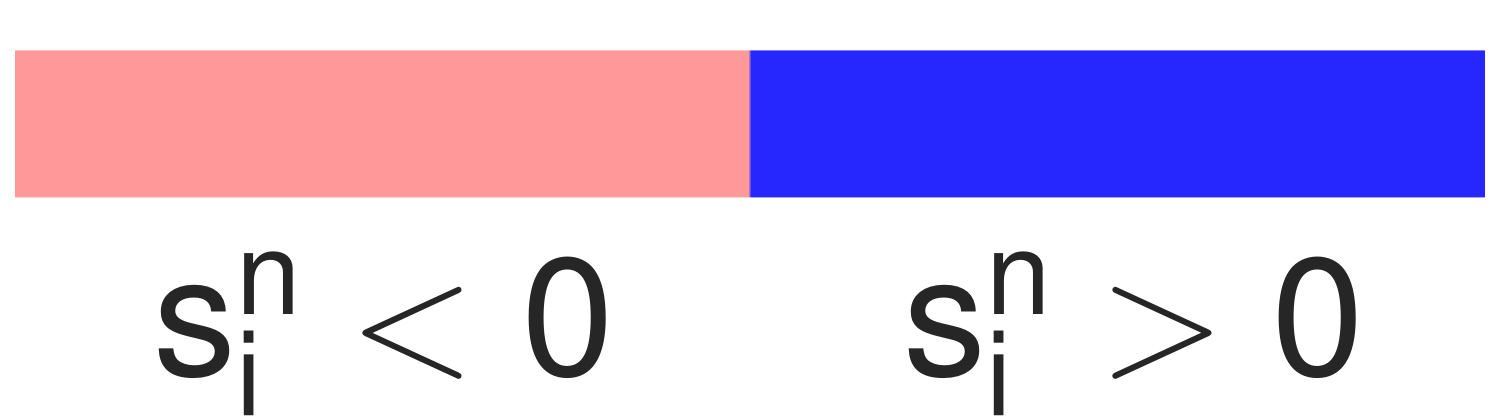
\includegraphics[trim=0 0 0 -2,width=4.0cm]{small_sign_s_cbar.png}}
\raisebox{5pt}{%
\begin{tcolorbox}[colframe=black,colback=white,boxrule=1.3pt,arc=3pt,left=2pt,right=2pt,top=2pt,bottom=2pt,boxsep=0pt,width=0.93cm]
    %\includegraphics[trim={0.8cm 0.8cm 0.8cm 0.8cm},clip,width=0.7cm]{example_squared_arena.png}
    \includegraphicsie[trim={0cm 0cm 0cm 0cm},clip,width=0.7cm]{annulus/2022-09-16_10-38-16/n180.pdf}
\end{tcolorbox} }
%\raisebox{-6pt}{\large Squared arena = diffusion has \textbf{converged}}
%\raisebox{-6pt}{\large Squared arena = diffusion has \textbf{converged}in sign to Fiedler vector (2nd eigenvector)}
\raisebox{15pt}{ \parbox{6.0cm}{\normalsize Squared arena = diffusion has\\[0pt]\textbf{converged} in sign\\[0pt]to the Fiedler vector $\textbf{v}_2$ }}
}
& \multicolumn{2}{|c|}{
\hspace{-0.60cm}
\raisebox{0.00\height}{
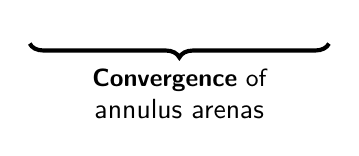
\begin{tikzpicture}[ultra thick]
\draw [decorate, decoration = {brace,raise=5pt,amplitude=5pt},line width=1.50pt]  (4.0,1.0) -- (0.2,1.0) node[pos=0.50,below=10pt,black]{\shortstack[c]{\small \textbf{Convergence} of\\annulus arenas}};
\end{tikzpicture}}
}
& \multicolumn{1}{|c|}{
\hspace{-0.50cm}
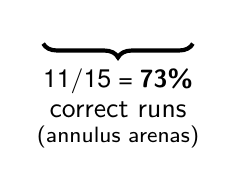
\begin{tikzpicture}[ultra thick]
%\draw [decorate, decoration = {brace,raise=5pt,amplitude=5pt},line width=1.50pt]  (2.2,1) -- (0.3,1) node[pos=0.50,below=10pt,black]{\shortstack[c]{\small Accuracy =\\\textbf{73\%} (30 runs)}};
    \draw [decorate, decoration = {brace,raise=5pt,amplitude=5pt},line width=1.50pt]  (2.2,1) -- (0.3,1) node[pos=0.50,below=10pt,black]{\shortstack[c]{\small $11/15 = \textbf{73\%}$\\correct runs\\\footnotesize(annulus arenas)}};
\end{tikzpicture}
}
\\[0cm]


\hline
\end{tabu}

\end{document}

